
\documentclass[12pt,a4paper]{article}
\usepackage[utf8]{inputenc} % sempre salve seus arquivos como UTF8
\usepackage[T1]{fontenc}
\usepackage[english]{babel}

\usepackage[left=2.5cm,right=2cm,top=2cm,bottom=2.5cm]{geometry}
\usepackage{amsmath}
\usepackage{amsthm}
\usepackage{amsfonts}
\usepackage{graphicx}
\usepackage{algorithm}
\usepackage{color}
\usepackage[noend]{algpseudocode}
\usepackage{mathtools}

% load times font
\usepackage{mathptmx}
\usepackage[scaled=.90]{helvet}
\usepackage{courier}

% comandos
\newcommand{\mdc}[1]{\mathrm{mdc}(#1)}

\DeclarePairedDelimiter\ceil{\lceil}{\rceil}
\DeclarePairedDelimiter\floor{\lfloor}{\rfloor}

% Foot without marker
\newcommand\blfootnote[1]{%
	\begingroup
	\renewcommand\thefootnote{}\footnote{#1}%
	\addtocounter{footnote}{-1}%
	\endgroup
}

\title{MO446 -- Introduction to Computer Vision  \\ Project 0}
\author{Breno Leite  \\ Guilherme Leite}
\date{10/08/2017}

\begin{document}

\maketitle
\blfootnote{\textit{\textbf{Important note:} The borders seen in the figures are not part of the image, they are figurative information about the starting and ending points of the image. Moreover, all the image scales in this report were changed in order to make the text more readable.}} \\

%% ---------------- Starts here --------------------------------

\textbf{Question 1.} \\

The Figure \ref{fig:p0-1-0} was used as an input to all the exercises, as specified it is a color image, rectangular and its type is \emph{PNG}. Th image dimensions are 400x300, which satisfies the required size. \\

\begin{figure}[!h]
	\centering
	{%
		\setlength{\fboxsep}{1pt}%
		\setlength{\fboxrule}{1pt}%
		\fbox{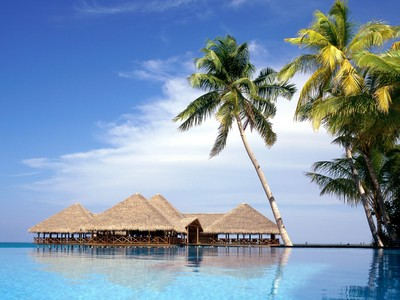
\includegraphics[scale=0.8]{input/p0-1-0}}%
	}%
	\caption{Input image used in the questions (\textbf{p0-1-0})}
	\label{fig:p0-1-0}
\end{figure}

\textit{Note:} The image was converted from \emph{JPG} to \emph{PNG} format. 

\newpage


\textbf{Question 2.} \\

\textbf{2-a) } A PNG image is represented in RGB format, which means that there is three channels for each pixel. These channels represents the intensity of each color, in a determined pixel, RGB stands for: Red, Green, and Blue. The Figure \ref{fig:p0-2-a-0} represents an image obtained by swapping the red and blue channel in the input image.


\begin{figure}[!h]
	\centering
	{%
		\setlength{\fboxsep}{1pt}%
		\setlength{\fboxrule}{1pt}%
		\fbox{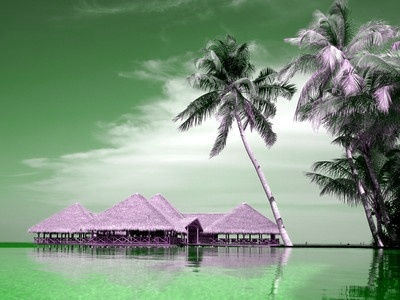
\includegraphics[scale=0.8]{output/p0-2-a-0}}%
	}%
	\caption{Input image with red and blue channels swapped (\textbf{p0-2-a-0})}
	\label{fig:p0-2-a-0}
\end{figure}

We can note a heavy intensity of green in the image after the swap, the reason for that is explained looking at the original image. Most of the pixels in the original image has a low intensity of red, in opposite, the intensity of blue is quite high mainly because of the water and sky. When the swap occurs, all the blue intensity goes to red highlighting things that had a little bit of red intensity on the original image, like the fences. \\

In other hand, all the intensity from the red (really low on the original image) goes to blue. So, that makes the intensity of blue goes down in places that blue was too high (e.g. water and sky). This way, the green color becomes more intense on places that blue was predominant on the original image, explaining the green lake.\\

\newpage


\textbf{2-b) } A monochrome or grayscale images is composed by a single channel, which ranges from 0 to 255 as RGB channels. Thus, create a monochrome image from the green channel is a straightforward procedure, it is just a copy of the green channel into a new image. The result obtained using this procedure on the input image is seen in the Figure \ref{fig:img-green}.

\begin{figure}[!h]
	\centering
	{%
		\setlength{\fboxsep}{1pt}%
		\setlength{\fboxrule}{1pt}%
		\fbox{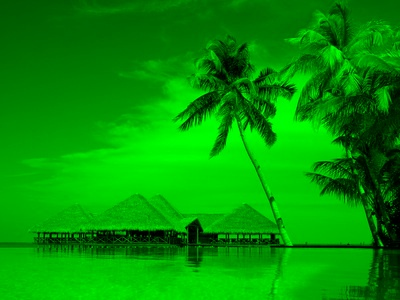
\includegraphics[scale=0.7]{output/p0-2-b-0}}%
	}%
	\caption{Monochrome image created from green channel (\textbf{p0-2-b-0})}
	\label{fig:img-green}
\end{figure}

As shown in the figure, the representation of the image stills really good. The reason for this is the high intensity of the green channel in the original image, which makes this channels, by its own, a good representation for image.\\

\textbf{2-c) } Using the same structure as in \textbf{2-c}, we this time use the red channel to create the new monochrome image, which is shown in Figure \ref{fig:img-red}.

\begin{figure}[!h]
	\centering
	{%
		\setlength{\fboxsep}{1pt}%
		\setlength{\fboxrule}{1pt}%
		\fbox{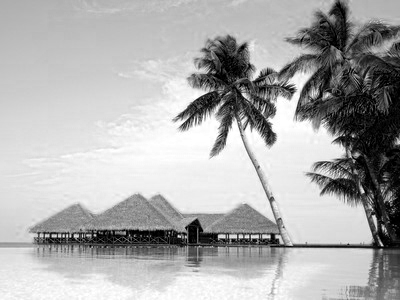
\includegraphics[scale=0.7]{output/p0-2-c-0}}%
	}%
	\caption{Monochrome image created from green channel (\textbf{p0-2-c-0})}
	\label{fig:img-red}
\end{figure}

In this image, we are able to see more blurred areas. The reason for this result is the low intensity of the red channel over the image pixels, which makes just the channel red not as good representation as the green channel.

\textbf{2-c) } The image created from the green channel looks more like what we expected, this is explained by the intensity of the three channels of the image. As said before, the original image is more intense on the green channel than in the red channel\footnote{Numbers to compare green and red channels (we need to collect that, maybe the mean of R and G?)}. We normally would expect to the green approach work better, mainly because the nature of the green color in the real world. However, we can not expect this result for every type of image. \\

\textbf{Question 3.} \\

\begin{figure}[!h]
	\centering
	{%
		\setlength{\fboxsep}{1pt}%
		\setlength{\fboxrule}{1pt}%
		\fbox{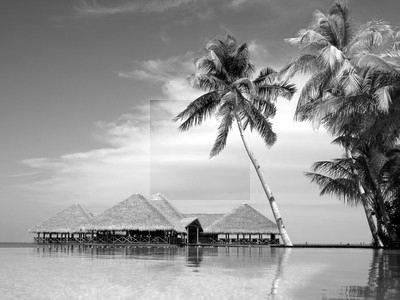
\includegraphics[scale=0.8]{output/p0-3-0}}%
	}%
	\caption{p0-3-0}
	\label{fig:p0-3-0}
\end{figure}


\begin{figure}[!h]
	\centering
	{%
		\setlength{\fboxsep}{1pt}%
		\setlength{\fboxrule}{1pt}%
		\fbox{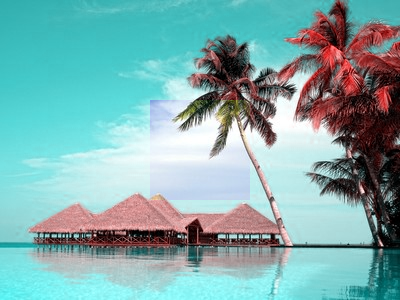
\includegraphics[scale=0.8]{output/p0-3-1}}%
	}%
	\caption{p0-3-1}
	\label{fig:p0-3-1}
\end{figure}


\begin{figure}[!h]
	\centering
	{%
		\setlength{\fboxsep}{1pt}%
		\setlength{\fboxrule}{1pt}%
		\fbox{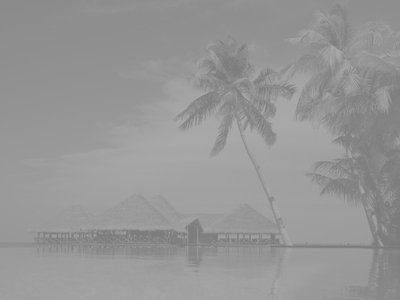
\includegraphics[scale=0.8]{output/p0-4-b-0}}%
	}%
	\caption{p0-4-b-0}
	\label{fig:p0-4-b-0}
\end{figure}


\begin{figure}[!h]
	\centering
	{%
		\setlength{\fboxsep}{1pt}%
		\setlength{\fboxrule}{1pt}%
		\fbox{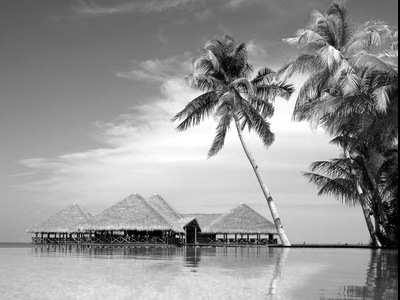
\includegraphics[scale=0.8]{output/p0-4-c-0}}%
	}%
	\caption{p0-4-c-0}
	\label{fig:p0-4-c-0}
\end{figure}

\begin{figure}[!h]
	\centering
	{%
		\setlength{\fboxsep}{1pt}%
		\setlength{\fboxrule}{1pt}%
		\fbox{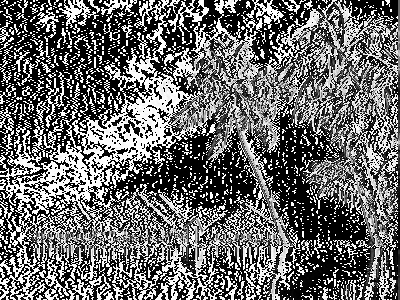
\includegraphics[scale=0.8]{output/p0-4-c-1}}%
	}%
	\caption{p0-4-c-1}
	\label{fig:p0-4-c-1}
\end{figure}


\begin{figure}[!h]
	\centering
	{%
		\setlength{\fboxsep}{1pt}%
		\setlength{\fboxrule}{1pt}%
		\fbox{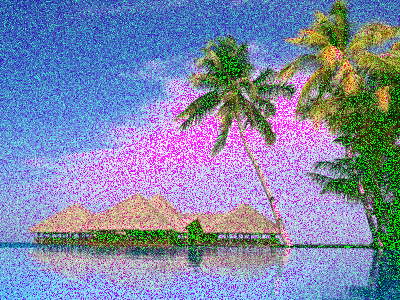
\includegraphics[scale=0.8]{output/p0-5-a-0}}%
	}%
	\caption{p0-5-a-0}
	\label{fig:p0-5-a-0}
\end{figure}

\begin{figure}[!h]
	\centering
	{%
		\setlength{\fboxsep}{1pt}%
		\setlength{\fboxrule}{1pt}%
		\fbox{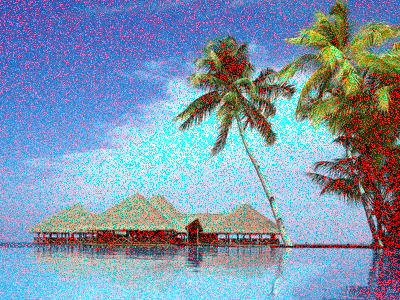
\includegraphics[scale=0.8]{output/p0-5-b-0}}%
	}%
	\caption{p0-5-b-0}
	\label{fig:p0-5-b-0}
\end{figure}


\end{document}

